% 请使用xelatex进行编译
\documentclass[12pt]{ctexart}

\pagestyle{empty}					
\setlength{\parindent}{0pt}			

\usepackage{enumitem}
\setitemize[1]{itemsep=4pt,partopsep=0pt,parsep=\parskip,topsep=5pt}

\usepackage{pifont}

\usepackage{marvosym}
\usepackage{textcomp}
\usepackage[top=1cm,left=1cm,right=1cm,bottom=1cm]{geometry}
\usepackage{graphicx}										
\usepackage{hyperref}
\usepackage{color}
\usepackage{setspace}
\definecolor{linkcolour}{rgb}{0,0.2,0.6}  
\hypersetup{colorlinks,breaklinks,urlcolor=linkcolour, linkcolor=linkcolour}
\usepackage[usenames,dvipsnames]{xcolor}					
%定义主题颜色
%建议与目标院校校徽颜色一致
\definecolor{ndz}{rgb}{0.5, 0.0, 0.5}%南大紫
\definecolor{tjl}{rgb}{0.0, 0.5, 1.0}%同济蓝
\definecolor{zdl}{rgb}{0.0, 0.18, 0.39}%浙大蓝
% 使用主题颜色
\newcommand{\myThemeColor}{tjl}

\newcommand{\boldnum}[1]{\textbf{\large\color{\myThemeColor}#1}}
\newcommand{\boldtext}[1]{\textbf{\color{\myThemeColor}#1}}

\newcommand{\cvsection}[1]
{\Large\color{\myThemeColor}\textbf{#1}\par
	\vspace{0.2cm}\normalsize\normalfont\normalcolor}

\newcommand{\cvitem}[1]
{\textbf{\color{\myThemeColor} #1}}

\newcommand{\itementry}[2]{	\vspace{0.5em}
	\hspace{0.7em}			
	\ding{72} \hspace{0.5em}\textbf{#1} \hfill      
	\color{\myThemeColor}#2 \normalsize\normalfont\normalcolor
	}
\newenvironment{newitem}{\itementry{}{}\\}{}

\begin{document}
\begin{spacing}{0.9}

\begin{minipage}[b]{5cm}
	% 以吴李为例
	\Huge\bfseries{\color{\myThemeColor}吴李}\normalsize\normalfont\\
	\\	\hspace{2em}
	\begin{tabular}{ll}
		本科院校:中国矿业大学    & 专业:***                    \\
		加权成绩:120         & 专业排名:\boldnum{1}/48(前3\%)                      \\
		电话:1550424454 & E-mail:234@cumt.edu.cn%尽量用学校邮箱	
	\end{tabular}
	\par\vspace{0pt}
\end{minipage}
	\hfill 
	\begin{minipage}[b]{3cm}
	% 插入证件照路径,最好白底,把路径fig/figure.jpg替换一下就好
		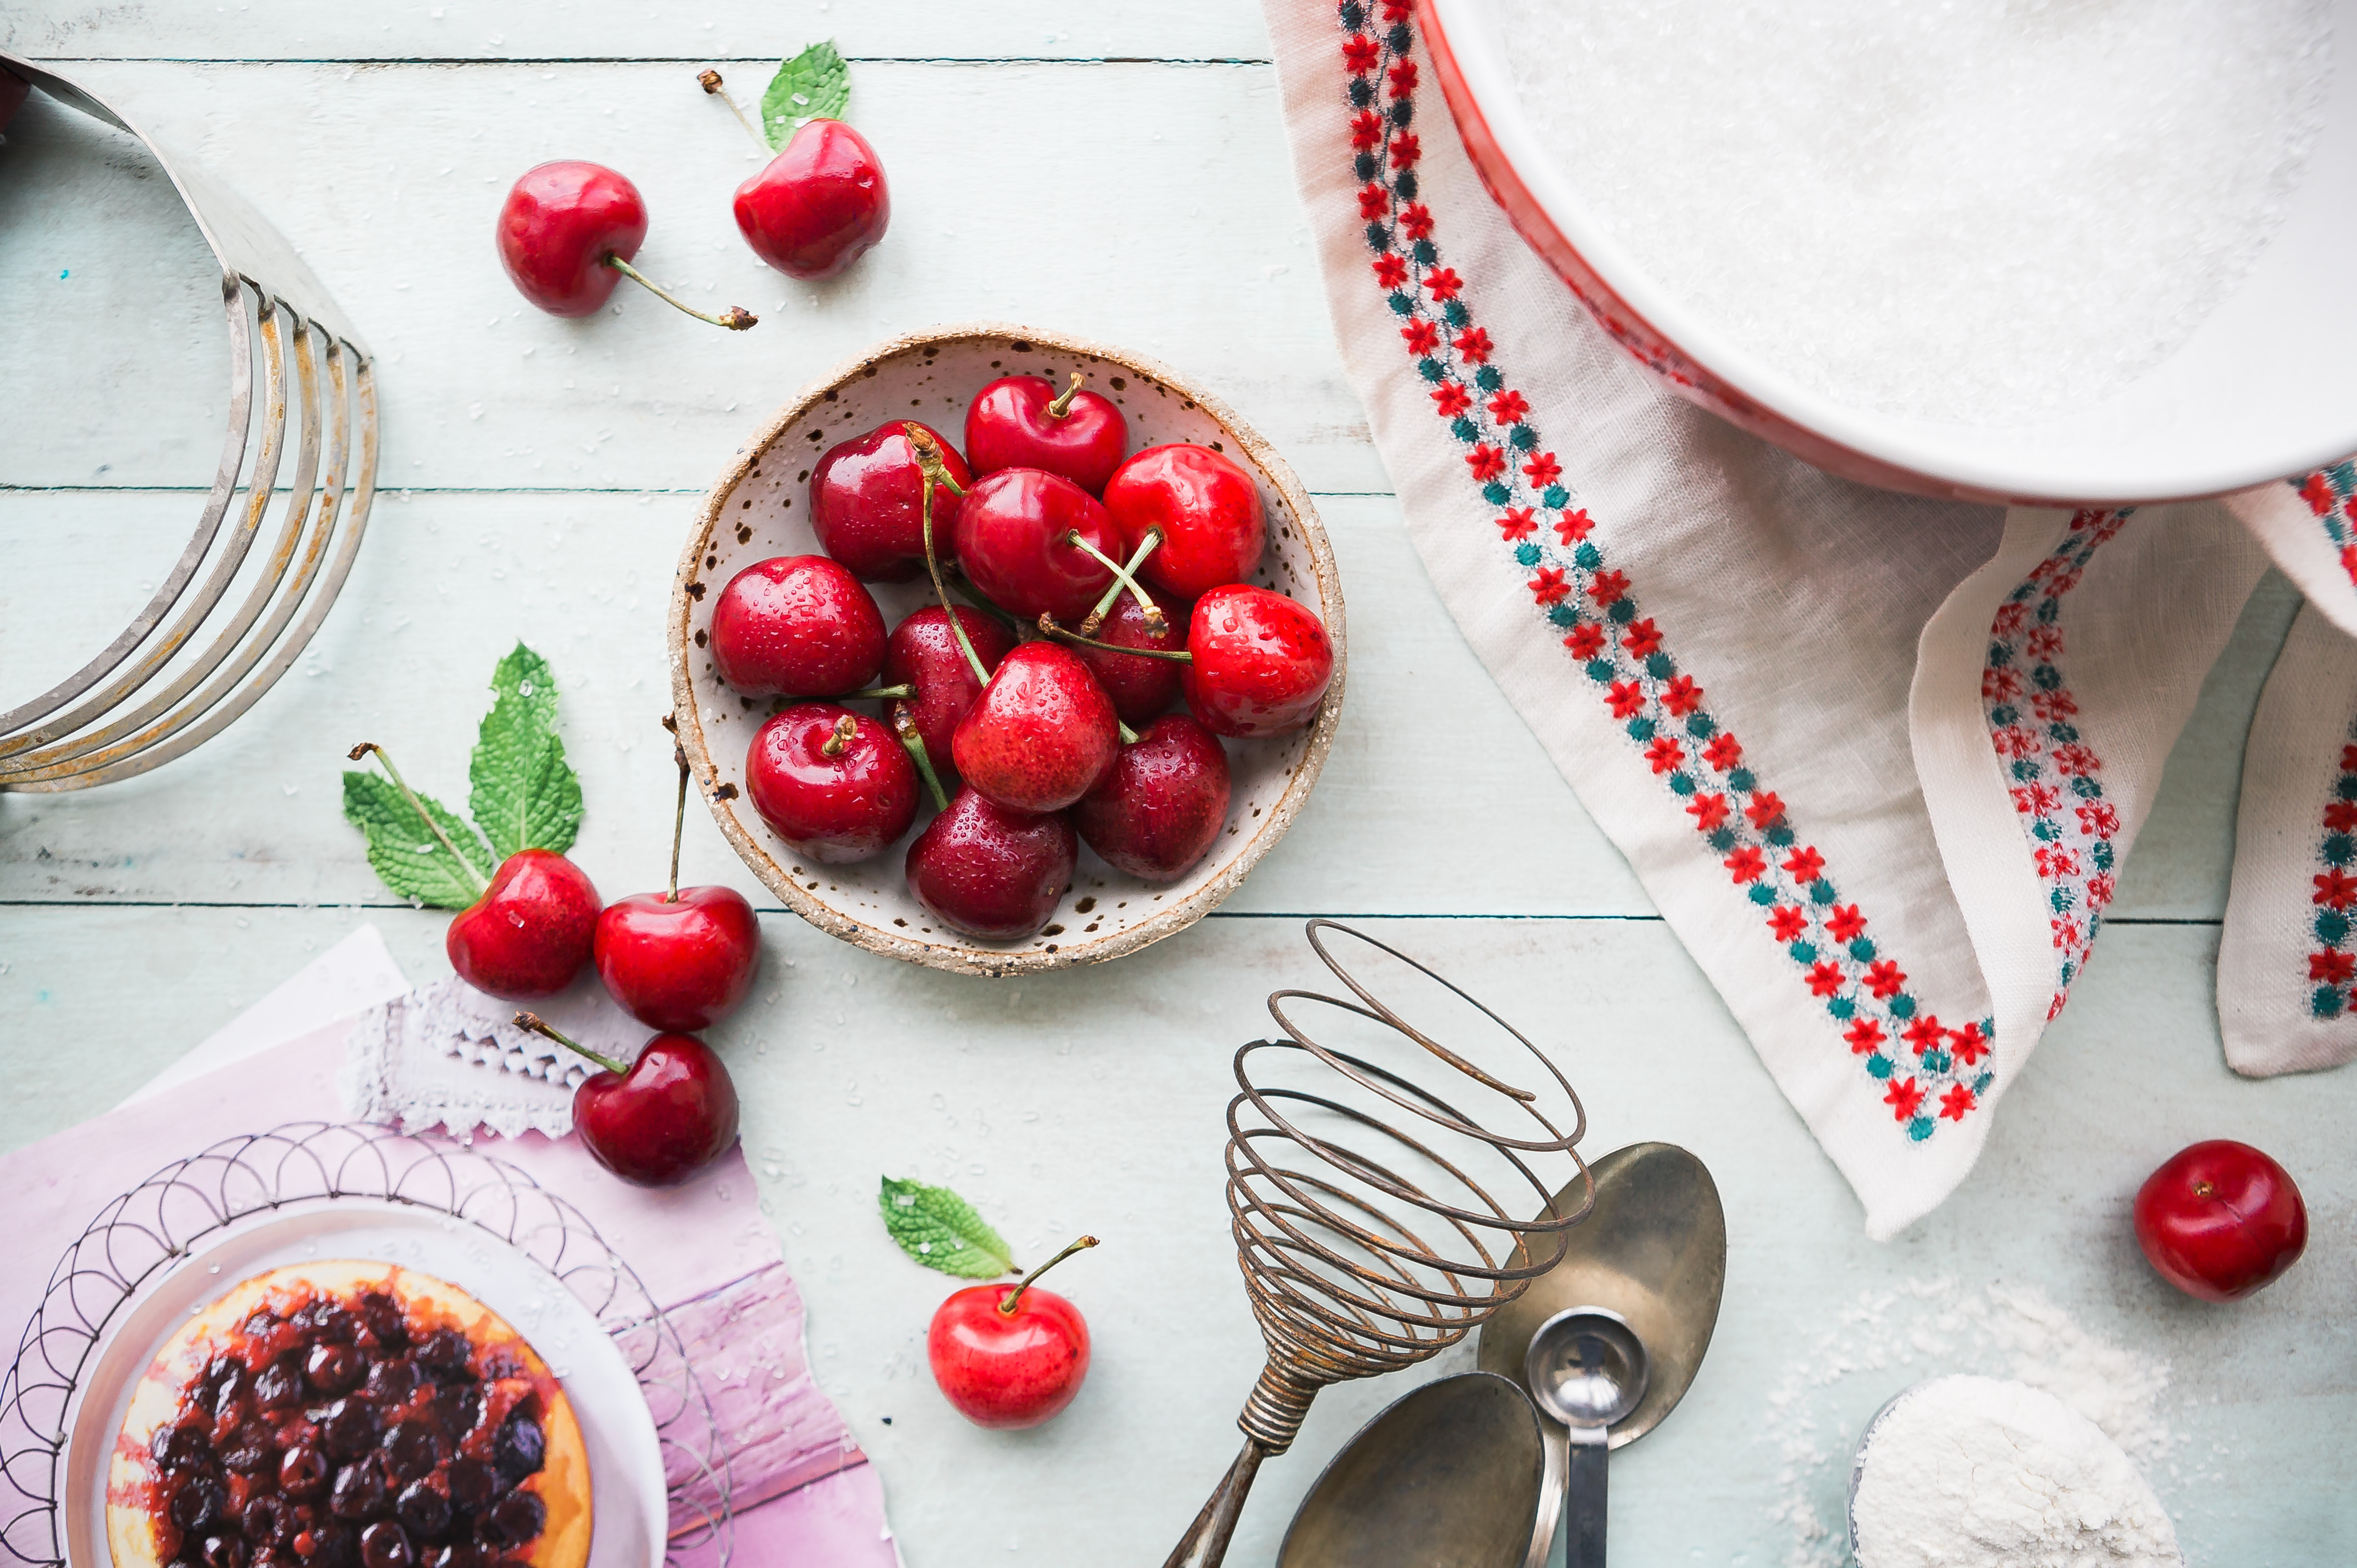
\includegraphics[width=2.0cm]{fig/figure.jpg}
		    \par\vspace{0pt}
	\end{minipage}
 \\
	\cvsection{\color{\myThemeColor}个人技能}
		\hrule
		\begin{itemize}
			\item[\ding{72}] 英语:CET-4(\boldnum{612}分),CET-6(\boldnum{562}分)
			\item[\ding{72}] 计算机:**** 
			\item[\ding{72}] 专业课程:***
			\item[\ding{72}] 其他方面:***
			\item[\ding{72}] ****
			\item[\ding{72}] ****
		\end{itemize}
	\cvsection{\color{\myThemeColor}科研竞赛}
		\hrule
	\begin{itemize}
		% 在每一条下边解释一下你的工作是什么,成果如何
		\item[\ding{72}] \textbf{主持项目****}\hfill
		\color{\myThemeColor}2019.4\\
		\normalsize\normalfont\normalcolor
		项目内容****,成果:以第一作者身份在北大核心期刊《**》上发表论文《***》
		\item[\ding{72}] 
		\textbf{****二等奖}\hfill
		\color{\myThemeColor}2019.4\\ \normalsize\normalfont\normalcolor
		....
		\item[\ding{72}] 
		\textbf{****一等奖}\hfill
		\color{\myThemeColor}2019.4\\ \normalsize\normalfont\normalcolor
		....
		\item[\ding{72}] 
		\textbf{****二等奖}\hfill
		\color{\myThemeColor}2018.4\\ \normalsize\normalfont\normalcolor
		....
		\item[\ding{72}] \textbf{****二等奖}\hfill
		\color{\myThemeColor}2018.6\\ 
		\normalsize\normalfont\normalcolor
		...

	\end{itemize}
	
	\cvsection{\color{\myThemeColor}其它奖项}
	\hrule
	\begin{itemize}
		\item[\ding{72}] **奖学金\hfill
		\color{\myThemeColor}2017.10 \normalsize\normalfont\normalcolor
		\item[\ding{72}] **比赛*等奖\hfill
		\color{\myThemeColor}2018.10 \normalsize\normalfont\normalcolor
		\item[\ding{72}] **奖\hfill
		\color{\myThemeColor}2017.10 \normalsize\normalfont\normalcolor
		\item[\ding{72}] **比赛*等奖\hfill
		\color{\myThemeColor}2017.10 \normalsize\normalfont\normalcolor
		\item[\ding{72}] **比赛*等奖\hfill
		\color{\myThemeColor}2017.10 \normalsize\normalfont\normalcolor
		\item[\ding{72}] **比赛*等奖\hfill
		\color{\myThemeColor}2017.10 \normalsize\normalfont\normalcolor
		\item[\ding{72}] **比赛*等奖\hfill
		\color{\myThemeColor}2017.10 \normalsize\normalfont\normalcolor
		\item[\ding{72}] **比赛*等奖\hfill
		\color{\myThemeColor}2017.10 \normalsize\normalfont\normalcolor
	\end{itemize}
	\cvsection{\color{\myThemeColor}自我评价}
	\hrule
	\vspace{1em}
	\hspace{2.5em}
	评价一下你自己
\end{spacing}
\end{document}